%%%%%%%%%%%%Loading Packages%%%%%%%%%%%%%%%%%%%%%%%%%%%%%%%
\documentclass{beamer}
\mode<presentation> \usetheme{Frankfurt}
\usepackage{hyperref}
\usepackage{rotating}
\usepackage{amsmath, amsthm, amssymb, amsfonts}
\usepackage{booktabs}
\usepackage[font=small, labelfont=bf]{caption}
%\setbeamercovered{transparent}
\usepackage{graphicx}
\usepackage{epsfig}
%\usepackage{tikz}
%\usepackage{xcolor}
%\usepackage{colortbl}
\setbeamertemplate{itemize items}[square]

\newcommand{\x}[1]{\alert{#1}}
%\definecolor{darkblue}{RGB}{0,0,139} % Defining dark blue color
%\newcommand{\filledsquare}{\tikz \draw[fill=darkblue] (0,0) rectangle (0.2,0.2);}

\begin{document}
\title{A Statistician’s Experience}
\author{Abidemi K. Adeniji, PhD\\ResTORbio, Inc.\\
	\bigskip
	\bigskip
	Presented to\\
	NESS-NextGen Data Science Day\\
	Yale University\\
	New Haven, CT\\
	October 27, 2018}
\frame{\titlepage}

%%%%Discalaimer%%%%%%%%%%%%%%%%%%%%
\begin{frame}
	\frame{\frametitle{Disclaimer}}
	\centering\textbf{\underline{Disclamer}}\\
	The materials presented are solely the views of the presenter\\
	Abidemi K. Adeniji.
\end{frame}

%%%%%%%%%%%%% Creating overview (table of contents)%%%%%%%%%%%%%%%%%%%
\begin{frame}
\frametitle{Overview}
\tableofcontents[hideallsubsections]
\end{frame}

%%%%%%%%%%%First section%%%%%%%%%%%%%%%%%%%%%%%%%%%%%%
\section{Preparation}
\frame{\frametitle{Outline}
\tableofcontents[currentsection, currentsubsection,hideallsubsections]}

%%%%%%%%%%%%%% First subsection for section one %%%%%%%%%%%%%%%%%%%%%%%%%%%%%%%%	
\subsection{School preparation}
\frame{\frametitle{Preparation}
	\tableofcontents[currentsection, currentsubsection]}

\begin{frame}
	\frame{\frametitle{School preparation}}
	\center
	\textbf{Public Speaking}\\
	\bigskip
	\begin{itemize}
		\item Actively seek opportunities to present.
		\begin{itemize}
			\item In group projects, ask to be the speaker.
		\end{itemize}
		\pause
		\item Learn how to tell your story.
	\end{itemize}	
\end{frame}


\begin{frame}
	\frame{\frametitle{School preparation}}
	\center
	\textbf{Public Speaking}\\
	\bigskip
	\begin{itemize}
		\item  Sign up for local clubs like Toastmasters
		\pause
			\begin{itemize}
				\item They are a leader in communication and leadership	development.
				\pause
				\item The bio-pharma market is changing, decisions are becoming
				more analytically driven giving statisticians more avenues for a
				sit at the table.
			\end{itemize}
	\end{itemize}
\end{frame}

\begin{frame}
	\frame{\frametitle{School preparation}}
	\center
	\textbf{Toastmasters locations in CT}
	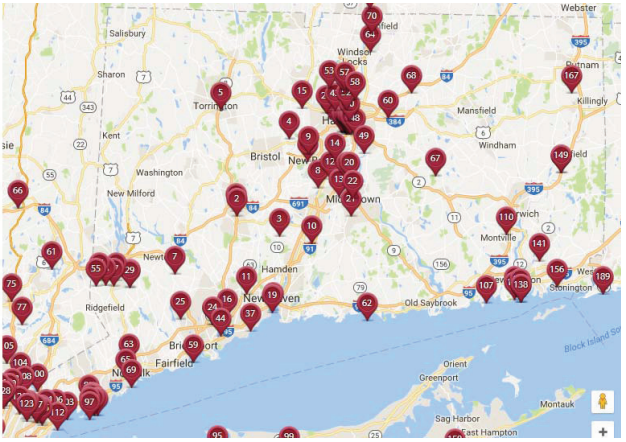
\includegraphics[width=0.70\textwidth]{toastmaster}
\end{frame}

\begin{frame}
	\frame{\frametitle{School preparation}}
	\center
	\textbf{Writing}\\
	\bigskip
	\begin{itemize}
		\item  Actively seek opportunities to write.
	\end{itemize}
	\pause
	\bigskip
	\textcolor{blue}{How to Write a Lot: A Practical Guide to Productive Academic
		Writing, P.J. Silvia, 2007}
\end{frame}

%%%%%%%%%%%%%% Second subsection for section one %%%%%%%%%%%%%%%%%%%%%%%%%%%%%%%%	
\subsection{Interview preparation}
\frame{\frametitle{Phone-screen interview}
	\tableofcontents[currentsection, currentsubsection]}
	
\begin{frame}
	\frame{\frametitle{Interview preparation}}
	\center
	\textbf{Recruiters}\\
	\pause
	\begin{itemize}
		\item  Recruiters can play an important role in getting you an interview.
		\item Recruiters can play an important role in getting you an interview.
		\begin{itemize}
			\item However, understand that the job of the recruiter is not to get
			you a job,\pause \alert {but to fill a position.}
		\end{itemize}
	\end{itemize}
\end{frame}
%%%%%%%%%%%%%%%%Second section%%%%%%%%%%%%%%%%%%%%%%%%%%%%%%%%%%%%%%%%%%%%%%%%%%%%%%
\section{On-site Interview}
\frame{\frametitle{Outline}
	\tableofcontents[currentsection, currentsubsection]}
\end{document}
